\documentclass[10pt]{article}
\makeatletter
\usepackage[numbered,autolinebreaks,useliterate]{mcode}
\usepackage{textcomp}
\usepackage{verbatim}
\usepackage{lmodern}
\usepackage{comment}
\excludecomment{Answ}
\usepackage{listings}
\usepackage{color} %red, green, blue, yellow, cyan, magenta, black, white
\definecolor{mygreen}{RGB}{28,172,0} % color values Red, Green, Blue
\definecolor{mylilas}{RGB}{170,55,241}
\renewcommand\paragraph{\@startsection{paragraph}{4}{\z@}%
            {-2.5ex\@plus -1ex \@minus -.25ex}%
            {1.25ex \@plus .25ex}%
            {\normalfont\normalsize\bfseries}}
\makeatother
\usepackage{gensymb}
\setcounter{secnumdepth}{4}
\usepackage{amsmath}
%\usepackage{mathtools}
\usepackage{graphicx}
\usepackage{slashed}
\usepackage{lineno}
\usepackage{latexsym}
\usepackage{subfigure}
\usepackage{amssymb}
\newtheorem{thm}{Theorem}[section]
\newtheorem{cor}[thm]{Corollary}
\newtheorem{lem}[thm]{Lemma}
\usepackage[numbers,sort]{natbib}
\usepackage{enumerate}
\newcommand{\bb}{\begin{equation}}
\newcommand{\ee}{\end{equation}}
\newtheorem{defin}{Definition}
\usepackage{multirow}
\usepackage{ctable}
\usepackage{bm}
\usepackage{enumerate}
\newcommand{\D}[2]{\frac{\partial #1}{\partial #2}}
\newcommand{\DD}[2]{\frac{\partial^2 #1}{\partial #2^2}}
\newcommand{\UB}[2]{\underbrace{#1}_{\textrm{\parbox{8em}{\centering #2}}}}
\newcommand{\rd}{\text{ d}}
\newcommand{\disk}{}
\usepackage{framed}
\newcommand{\see}[1]{(see Figure \ref{#1})}
\newcommand{\fig}[1]{Figure \ref{#1}}
\newcommand{\figs}[2]{figures \ref{#1} and \ref{#2}}
\newcommand{\sect}[1]{Section \ref{#1}}
\newcommand{\app}[1]{Appendix \ref{#1}}
\newcommand{\chap}[1]{Chapter \ref{#1}}
\newcommand{\eqn}[1]{equation \eqref{#1}}
\newcommand{\eqns}[2]{equations \eqref{#1} and \eqref{#2}}
\newcommand{\eqnto}[2]{equations \eqref{#1}-\eqref{#2}}
%\usepackage{authblk}
\usepackage{url}
\usepackage{hyperref}
\usepackage{soul}
\newcommand{\eg}{\emph{e.g.} }
\newcommand{\bn}{\bm{n}}
\newcommand{\bu}{\bm{u}}
\newcommand{\ie}{\emph{i.e.} }
\newcommand{\Chapter}[1]{\chapter{#1}\label{#1}}
\newcommand{\Section}[1]{\section{#1}\label{#1}}
\newcommand{\Subsection}[1]{\subsection{#1}\label{#1}}
\newcommand{\Subsubsection}[1]{\subsubsection{#1}\label{#1}}
\newcommand{\Appendix}[1]{\appendix{#1}\label{#1}}
\usepackage[margin=1.5cm,centering]{geometry}
\usepackage[geometry]{ifsym}
\makeatletter
\newcommand\restr[2]{{% we make the whole thing an ordinary symbol
  \left.\kern-\nulldelimiterspace % automatically resize the bar with \right
  #1 % the function
  \vphantom{\big|} % pretend it's a little taller at normal size
  \right|_{#2} % this is the delimiter
  }}
\def\url@leostyle{%
  \@ifundefined{selectfont}{\def\UrlFont{\sf}}{\def\UrlFont{\small\ttfamily}}}
\makeatother
\urlstyle{leo}
\usepackage{multirow}
\usepackage{blkarray}
\usepackage{soul}
\usepackage{framed}
\usepackage{color}
\usepackage{setspace}
\newcommand{\ttttp}{.24\textwidth}
\newcommand{\tttp}{.32\textwidth}
\newcommand{\ttp}{.45\textwidth}
\newcommand{\tp}{.8\textwidth}
\newcommand{\tbo}{.6\textwidth}
 \usepackage[T1]{fontenc}
\usepackage[utf8]{inputenc}
\usepackage{authblk}
 \renewcommand{\l}{\left(}
\renewcommand{\r}{\right)}
%\begin{figure}[h!!!tb]
%\centering
%\subfigure[\label{Godzilla}]{\includegraphics[height=0.35\textwidth]{./Pictures/Godzilla_final_bw.png}}
%\subfigure[\label{Jaeger}]{\includegraphics[height=0.35\textwidth]{./Pictures/Jaeger_finish_bw.png}}
%\caption{\label{Monsters} The two types of monster we are going to consider are: (a) the naturally occurring Kaijus and (b) the man-made Jaegers.}
%\end{figure}
\newcounter{Counter1}

\begin{document}

\lstset{language=Matlab,%
    %basicstyle=\color{red},
    breaklines=true,%
    morekeywords={matlab2tikz},
    keywordstyle=\color{blue},%
    morekeywords=[2]{1}, keywordstyle=[2]{\color{black}},
    identifierstyle=\color{black},%
    stringstyle=\color{mylilas},
    commentstyle=\color{mygreen},%
    showstringspaces=false,%without this there will be a symbol in the places where there is a space
    numbers=left,%
    numberstyle={\tiny \color{black}},% size of the numbers
    numbersep=9pt, % this defines how far the numbers are from the text
    emph=[1]{for,end,break},emphstyle=[1]\color{red}, %some words to emphasise
    %emph=[2]{word1,word2}, emphstyle=[2]{style},    
}


\title{Problem sheet 5}
\author{Thomas E. Woolley\\Last edited on:}
\maketitle
\section{Fixing the logistic map}\label{Fixing the logistic map}
One of the big problems with the discrete logistic equation is that if your initial population is too high then the population will become negative, namely, you can never start with more than the carrying capacity. Many equations have been suggested to correct for this phenomena. We will be investigating the following:
\bb
x_{n+1}=f(x_n)=\frac{\mu^3 x_n}{(1+x_n)^3},\label{Inverse_cubic}
\ee
where $\mu$ is a positive constant.
\begin{enumerate}
\item Draw a sketch of $(x,f(x))$ and $(x,x)$ on the same axes. How many non-negative steady states do we expect?

\item Derive the non-negative steady states, noting any parameter dependencies.\label{ststq}

\item Derive the stability of the steady states, noting any parameter dependencies.

\item Show that period two oscillatory points, $x_p$, satisfy
\bb
\l 1+x_p \r \l 1+\frac {\mu^3 x_p}{ \l 1+x_p \r^3} \r=\mu^2.\label{xp}
\ee

\item Solve for $x_p$ by following the proceeding steps.
\begin{enumerate}

\item Rewrite \eqn{xp} as a cubic in $y=1+x_p$.

\item Note that $x_s=\mu-1$ is a steady state (that should have found in question \ref{ststq}) and remember that any steady state is also a solution of \eqn{xp}. Using this knowledge rewrite the cubic in $y$ in the form
\bb
(y-\mu)(y^2+ay+b)=0
\ee 
where $a$ and $b$ should be defined in terms of $\mu$.

\item Solve $y^2+ay+b=0$ and hence derive $x_p$, noting any parameter dependencies.

\item Calculating the stability of the period two states is very hard to do by hand. However, explain how it would be done. Namely, define the inequality that would have to be calculated.

\item The bifurcation diagram of \eqn{Inverse_cubic} is shown in \fig{Discrete_inverse_cubic}, note the logarithmic $y$-axis. Explain what it shows and how it compares with the results you have generated in this question.
\begin{figure}[h!!!tb]
\centering
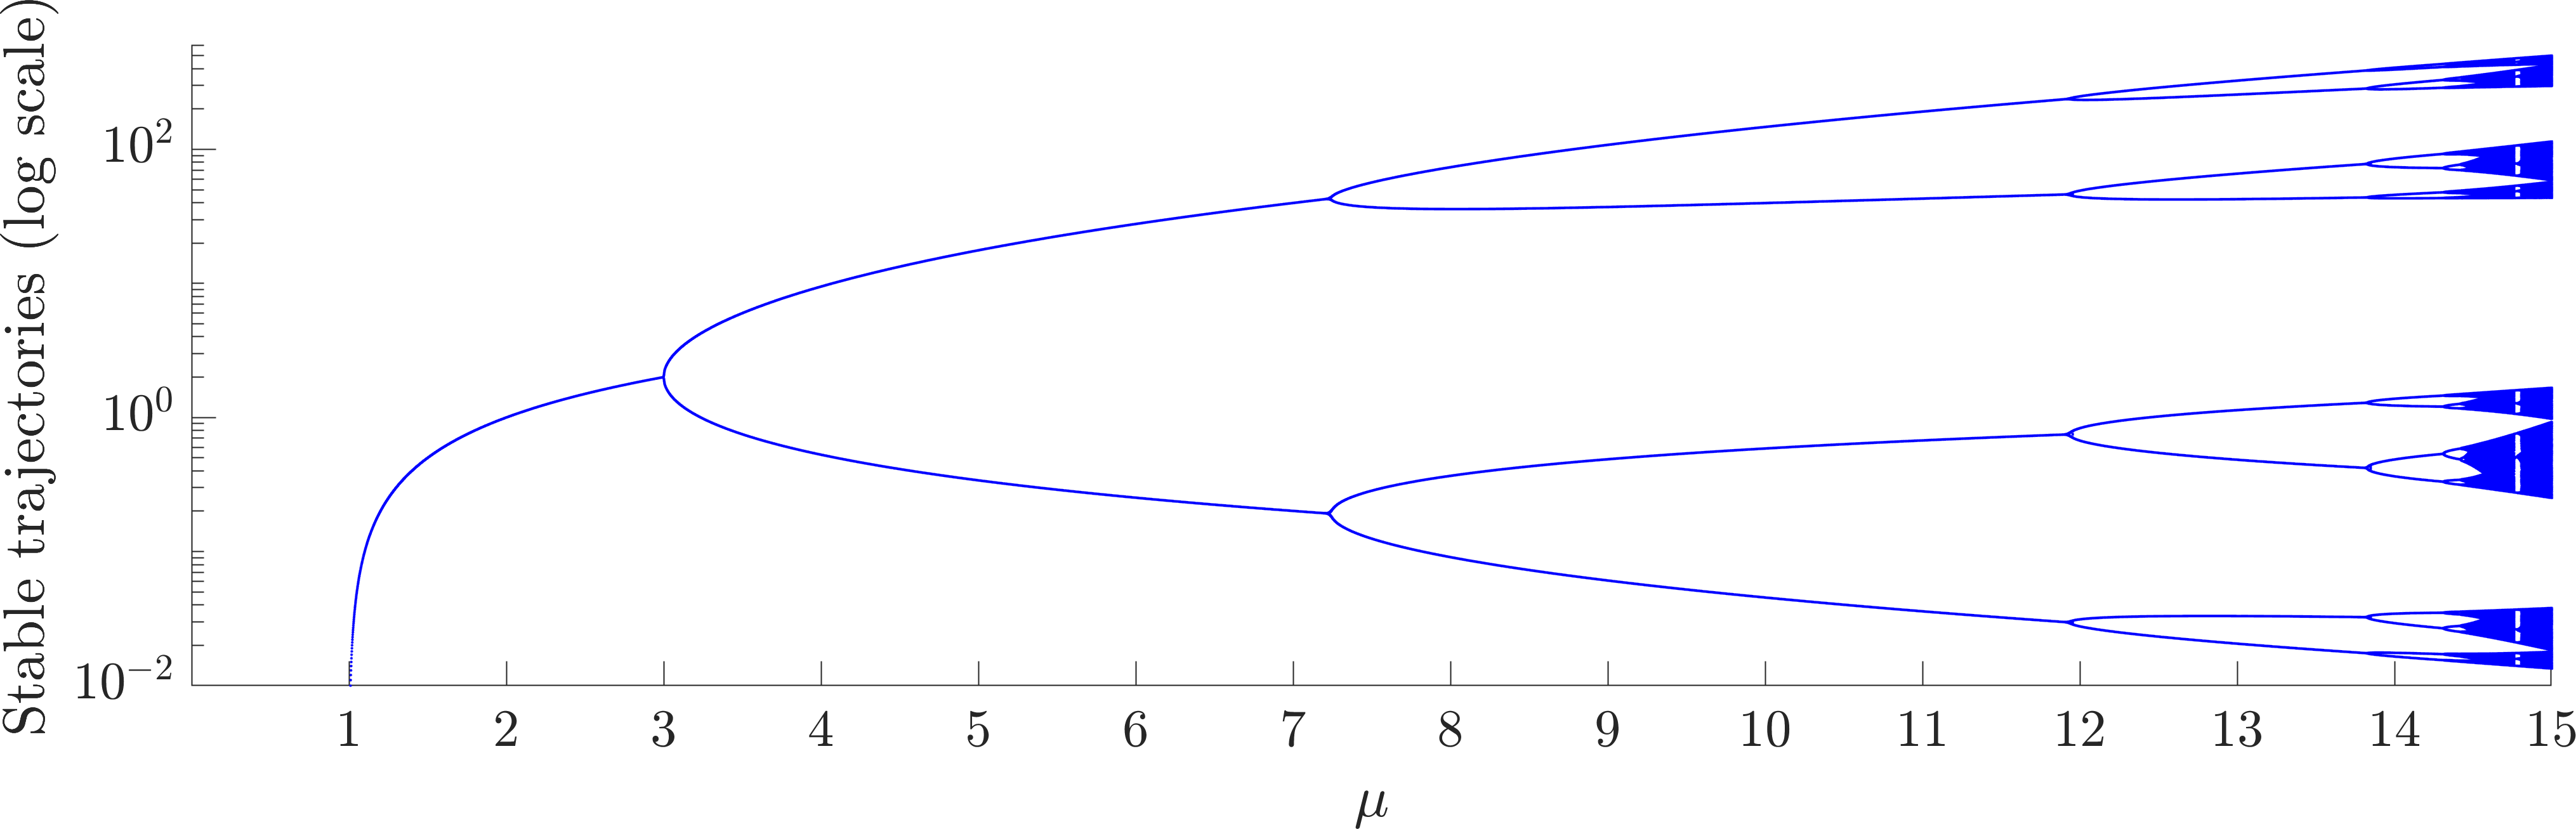
\includegraphics[width=\textwidth]{../../Pictures/Discrete_inverse_cubic.png}
\caption{\label{Discrete_inverse_cubic} Bifurcation diagram of \eqn{Inverse_cubic}, note the logarithmic $y$-axis.}
\end{figure}
\end{enumerate}

\end{enumerate}




\begin{Answ}
\subsection{Answers}
\begin{enumerate}
\item From \fig{Discrete_schematic} we expect 2 steady states, one zero and one positive.
\begin{figure}[h!!!tb]
\centering
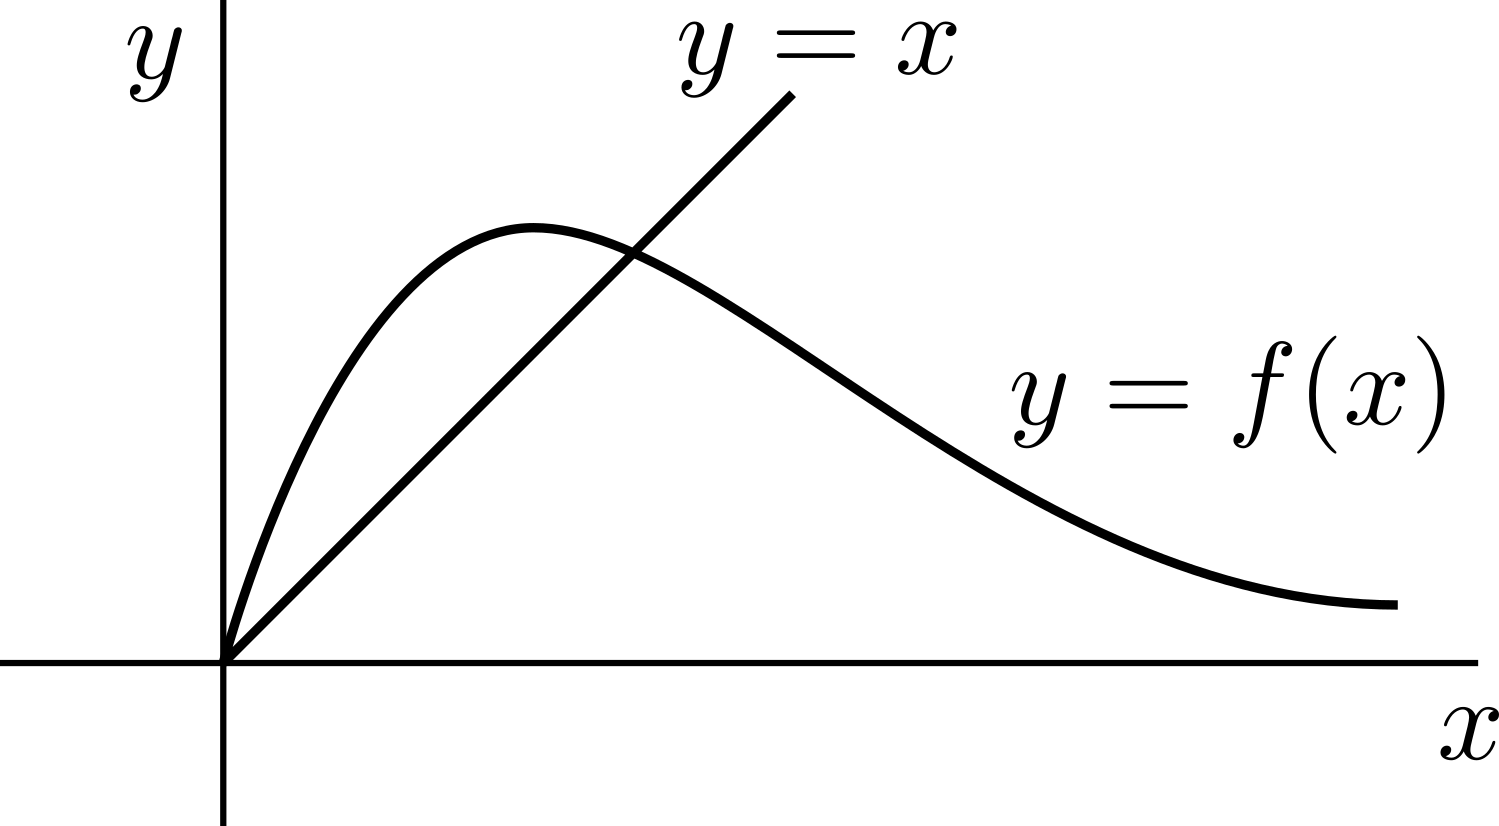
\includegraphics[width=\ttp]{../../Pictures/Discrete_schematic.png}
\caption{\label{Discrete_schematic} Plot of $(x,f(x))$ and $(x,x)$.}
\end{figure}

\item The steady states satisfy $x_n=x_s$ for all $n$. Thus
\bb
x_s=\frac{\mu^3 x_s}{(1+x_s)^3},
\ee
which implies $x_{s0}=0$ is a steady state and
\bb
(1+x_s)^3=\mu^3, \implies x_{s1}=\mu-1,
\ee
is another. Notably, $\mu\geq 1$ is required for the steady state to exist in the positive quadrant.

\item To calculate the stability we need to obtain the derivative of $f$,
\bb
f'(x)=\frac{\mu^3}{ \l 1+x \r^3}-\frac{3\mu^3 x}{ \l 1+x \r^4},
\ee
then evaluate $f'$ at the steady states and compare $|f'(x_s)|$ to one.

Since $f'(0)=\mu^3$ then
\bb
x_s\textrm{ is }\left\{\begin{array}{l}
\textrm{ stable for } \mu<1,\\
\textrm{ unstable for } \mu>1.
\end{array}\right.
\ee

Equally, we consider
\begin{align}
&|f'(\mu-1)|<1,\nonumber\\
\implies &-1<f'(\mu-1)<1,\nonumber\\
\implies & -1<1-\frac{3(\mu-1)}{\mu}<1,\nonumber\\
\implies & 2>\frac{3(\mu-1)}{\mu}>0,\nonumber\\
\implies & 2\mu>3\mu-3>0,\nonumber\\
\implies & 3>\mu>1.\nonumber
\end{align}
Thus, $x_{s1}$ is stable for $1<\mu<3$.


\item The period two points satisfy $x_p=f(f(x_p))$,
\bb
x_p={\frac {{\mu}^{6}x_p}{ \left( 1+x_p \right) ^{3} \left( 1+{\frac {{\mu}^{3}x_p}{ \left( 1+x_p \right) ^{3}}} \right) ^{3}}}.
\ee
We can cancel the $x_p=0$ root as it is a steady state $x_{s0}$. Further, we can take a cube root and multiply by the denominator to get \eqn{xp}.

\item 
\begin{enumerate}
\item Defining $y=1+x_p$ gives
\bb
y\l 1+\frac{\mu^3(y-1)}{y^3}\r=\mu^2,
\ee
which is
\bb
y^3-\mu^2y^2+\mu^3y-\mu^3=0,\label{y_cubic}
\ee
upon rearrangement.
\item We now want to factorise \eqn{y_cubic}. As mentioned in the question $y=\mu$ is a root (substitute $y=\mu$ into \eqn{y_cubic} to demonstrate this), so we know that we can rewrite \eqn{y_cubic} as
\bb
(y-\mu)(y^2+ay+b)=y^3-\mu^2y^2+\mu^3y-\mu^3.
\ee
Expanding the left-hand side and comparing terms by inspection we discover that $b=\mu^2$ and $a=\mu-\mu^2$, so
\bb
(y-\mu)(y^2+(\mu-\mu^2)y+\mu^2)=y^3-\mu^2y^2+\mu^3y-\mu^3.\label{y_factored}
\ee

\item Solving the quadratic term in \eqn{y_factored} gives
\bb
2y_\pm=\mu^2-\mu\pm\sqrt{\l\mu^2-\mu\r^2-4\mu^2},
\ee
or
\bb
x_{p\pm}=\frac{\mu^2-\mu-2\pm\sqrt{\l\mu^2-\mu\r^2-4\mu^2}}{2}.
\ee
Critically, we require $x_{p\pm}$ to be real and positive. Hence, we require
\bb
\mu^2-\mu-2>0, \implies (\mu+1)(\mu-2)>0,\label{ineq2}
\ee
so $\mu>2$. And we require
\bb
\l\mu^2-\mu\r^2-4\mu^2>0, \implies \mu^2-\mu>2\mu \textrm{ or }  \mu^2-\mu<-2\mu
\ee
Since $\mu^2-\mu<-2\mu$ implies $\mu^2<-\mu$, which is impossible, we must satisfy
\bb
\mu^2-\mu>2\mu, \implies \mu^2>3\mu, \implies \mu>3.
\ee
Thus although we derived the inequality $\mu>2$ through inequality \eqref{ineq2} we have to satisfy $\mu>3$ which is the the stronger requirement. Thus, in conclusion, the periodic two oscillatory states are
\bb
x_{p\pm}=\frac{\mu^2-\mu-2\pm\sqrt{\l\mu^2-\mu\r^2-4\mu^2}}{2}.
\ee
and appear for $\mu>3$.

\item The stability of $x_\pm$ is found by considering the size of $\lambda(x)=|\rd f(f(x))/\rd x|$. If $\lambda(x_{p\pm})>1$ the oscillatory trajectory is unstable. Alternatively, if $\lambda(x_{p\pm})<1$ the oscillatory trajectory is stable.

\item First we note that since we are on a log scale we cannot visualise the $x_{s0}=0$ steady state. However, we know that $x_{s0}$ is stable for $\mu<1$. At $\mu=1$ there is a bifurcation and $x_{s0}$ becomes unstable whilst $x_{s1}$ becomes stable for $1<\mu<3$. At $\mu=3$ the steady state destabilises to a periodic two trajectory $x_{p\pm}$, which is stable between $3<\mu \lesssim 7.5$ (by considering the \fig{Discrete_inverse_cubic}). Using an algebraic solver we can find that the period two oscillatory trajectory is stable for $3<\mu<3+3\sqrt{2}=\approx 7.24$. Continuing on, using \fig{Discrete_inverse_cubic}, we see that the period of the stable oscillations doubles with increasing $\mu$ until eventually chaos is seen for $\mu>14$.
\end{enumerate}


\end{enumerate}
\end{Answ}

\section{Squirrels}\label{Squirrels}
\begin{figure}[h!!!tb]
\centering
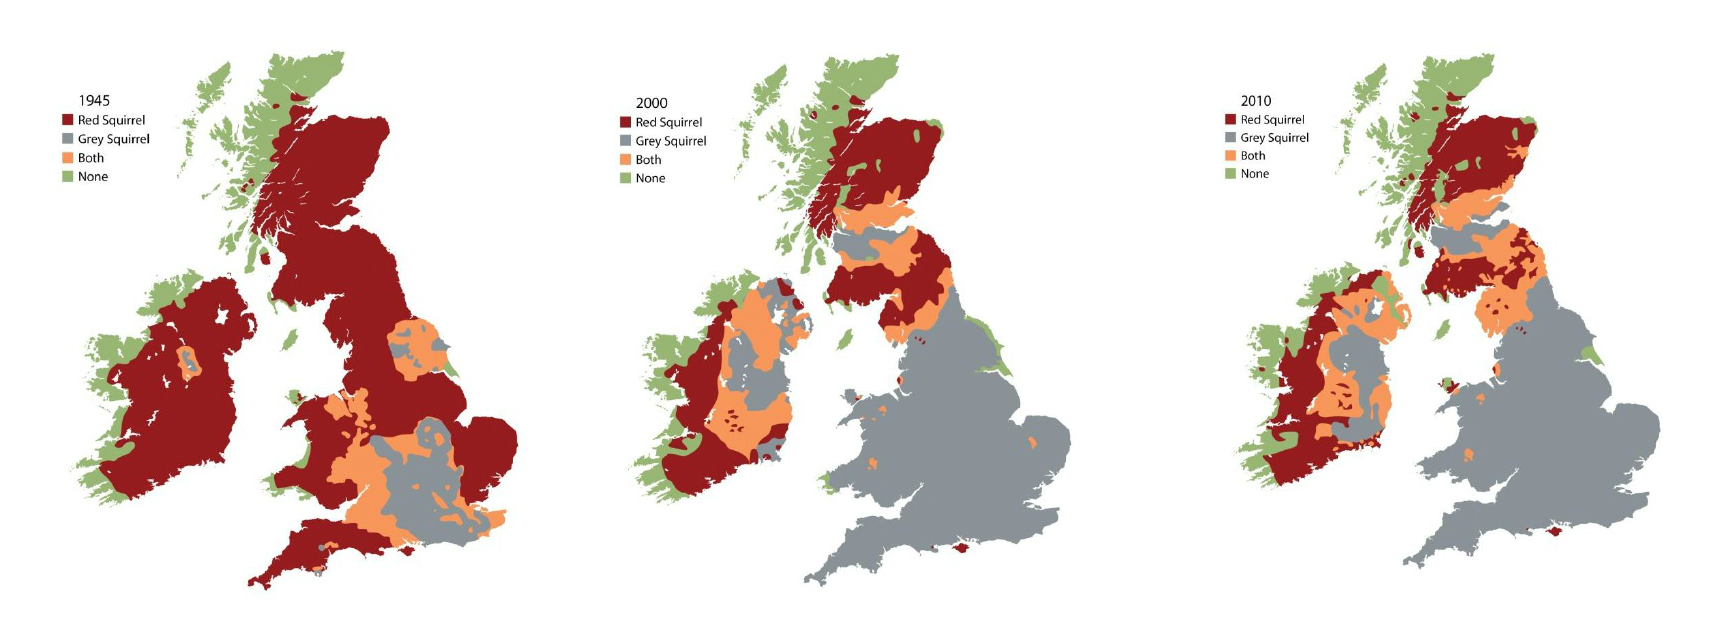
\includegraphics[width=\textwidth]{../../Pictures/SquirrelMap.png}
\caption{\label{SquirrelMap} Evolution of the spatial distribution of red and grey squirrels over time from the UK government's \href{https://aphascience.blog.gov.uk/2018/10/09/red-squirrel/}{science blog}.}
\end{figure}
Consider an infinite one-dimensional domain, in which Grey, $G$, and red, $R$, squirrel populations undergo the following interactions:
\begin{itemize}
\item Both Grey and Red squirrel populations move randomly through their domains with rates $D_G$ and $D_R$, respectively.
\item Grey squirrels are born at a rate proportional to their population, where the proportionality constant is $b_1$.
\item Red squirrels are born at a rate proportional to their population, where the proportionality constant is $b_2$.
\item Both squirrel populations compete internally with members of their own population (\ie grey compete with grey and red compete with red, respectively). Namely, whenever two members of the same population interact one of the members is suppressed. The constant of proportionality is $d_1$ for the grey squirrels and $d_2$ for the red squirrels.
\item The squirrels also compete across species. Namely, a grey and a red squirrel interaction can lead to a reduction in red squirrels, or a reduction in grey squirrels. The rate of proportionality for the reduction of grey squirrels is $c_1$, whilst the rate of proportionality for the reduction of red squirrels is $c_2$.
\end{itemize}

\begin{enumerate}
\item Ignoring movement for a moment, write down the interaction equations specified by the above description.


\item Show that the interaction equations and movement description lead to the following PDEs,
\begin{align}
\D{G}{t}&=D_G\DD{G}{x}+b_1G-d_1G^2-c_1RG,\label{G}\\
\D{R}{t}&=D_R\DD{R}{x}+b_2R-d_2R^2-c_2RG.\label{R}
\end{align}

\item Non-dimensionalise the system to produce the following equations,
\begin{align}
\D{u}{\tau}=&\DD{u}{X}+u(1-u-\alpha_{12}v),\label{u}\\
\D{v}{\tau}=&D\DD{v}{X}+\rho v(1-v-\alpha_{21}u).\label{v}
\end{align}


\item What are the parameter groupings $D$, $\rho$, $\alpha_{12}$ and $\alpha_{21}$ in terms of $b_1$, $b_2$, $d_1$, $d_2$, $c_1$ and $c_2$?

\item Find all homogeneous steady states of the system, noting any parameter dependencies that need to be satisfied for the steady state to exist.

\item Calculate the stability of the trivial homogeneous  steady states. Namely, those in which one of the populations is zero, noting parameter dependencies of the stability criterion.

Hint: you should find there are four cases:
\begin{enumerate}
\item $\alpha_{12}<1$ and $\alpha_{21}<1$;
\item $\alpha_{12}<1$ and $\alpha_{21}>1$;
\item $\alpha_{12}>1$ and $\alpha_{21}<1$;
\item $\alpha_{12}>1$ and $\alpha_{21}>1$.
\end{enumerate}
\setcounter{Counter1}{\value{enumi}}
\end{enumerate}


Calculating the stability of the fourth steady state,
\bb
(u_s,v_s)=\frac{1}{1-\alpha_{12}\alpha_{21}}(1-\alpha_{12},1-\alpha_{21}),
\ee
leads to a complicated eigenvalue calculation and we will use curve sketching in the next question to consider the stability of this steady state.



\begin{enumerate}
\setcounter{enumi}{\value{Counter1}}
\item Sketch the $(u,v)$ phase plane in each of the cases (a)-(d). You should include: the nullclines; annotations regarding the signs of $\rd u/\rd \tau$ and $\rd v/\rd \tau$ in each region delineated by the nullclines; accompanying directional arrows in each region; directional arrows on the nullclines; and, finally, trajectories illustrating the expected evolution with initial conditions taken from each region.

Use these sketches to determine the stability of $(u_s,v_s)$, when it exists.
\item Describe what happens to the grey and red squirrels in each of the cases (a)-(d).\label{Squirrel_param_region}

\item By considering \fig{SquirrelMap} and question \ref{Squirrel_param_region} what parameter region do you think we are in?

\item Can the non-zero steady state, $(u_s,v_s)$, undergo a Turing instability?
\setcounter{Counter1}{\value{enumi}}
\end{enumerate}

Now suppose we fix some constants and begin to consider the spatial aspects of the problem. Namely let $D=1$, $\rho=1$, $\alpha_{12}=1/2$, $\alpha_{21}=3/2$.  Further, suppose we supply the boundary conditions $u(-\infty)=1$, $v(-\infty)=0$ and $u(\infty)=0$, $v(\infty)=1$ and initial condition $u=0$, $v=1$ almost everywhere.

\begin{enumerate}
\setcounter{enumi}{\value{Counter1}}
\item What do these parameters, boundary and initial conditions mean in terms of the biology of the problem?

\item  Provide a guess as to how the population will evolve.\label{question}

\item Convert \eqns{u}{v} into a moving frame of reference by converting the coordinates $(X,\tau)$ into $(z,\tau)$ where $z=X-c\tau$ and $c$ is a positive constant.

\item If we define $s=u+v$ then show that travelling wave with a stationary profile satisfies
\bb
0=\frac{\rd^2 s}{\rd z^2}+c\frac{\rd s}{\rd z}+s(1-s),\label{s}
\ee
where you should also specify the boundary and initial conditions.

\item By inspection offer a simple solution to \eqn{s}.

\item Deduce that, under the given conditions,
\bb
0=\frac{\rd^2 u}{\rd z^2}+c\frac{\rd u}{\rd z}+(1-\alpha_{12})u(1-u)\label{u_solo}.
\ee


\item Show that \eqn{u_solo} can support a travelling wave solution if $c\geq 2\sqrt{1-\alpha_{12}}$.


\item Having looked at \eqns{G}{R} in a number of ways return to question \ref{question}. Have your thoughts about the spatio-temporal evolution of the red and grey squirrel populations changed? Does this model represent what is happening in \fig{SquirrelMap}?
\end{enumerate}



\begin{Answ}
\subsection{Answers}
\begin{enumerate}
\item \label{Interaction_equations}
\begin{align}
G&\mathrel{\mathop{\rightleftarrows}^{b_1}_{d_1}}2G,\quad G+R\stackrel{c_1}{\rightarrow}R.\\
R&\mathrel{\mathop{\rightleftarrows}^{b_2}_{d_2}}2R,\quad G+R\stackrel{c_2}{\rightarrow}G.
\end{align}

\item Using the Law of Mass Action on the interactions equations shown in answer \ref{Interaction_equations} and adding diffusive movement to the system we get \eqns{G}{R}.

\item Using $G=[G]u$, $R=[R]v$, $x=[x]X$ and $t= [t]\tau$ we find that $[G]=b_1/d_1$, $[R]=b_2/d_2$, $[x]=\sqrt{D_G/b_1}$ and $[t]=1/b_1$. 

\item Subsequently, $D=D_R/D_G$, $\rho=b_2/b_1$, $\alpha_{12}=c_1b_2/(d_2b_1)$ and $\alpha_{21}=c_2b_1/(d_1b_2)$.

\item The steady states are (0,0), (0,1), (1,0) and
\bb
(u_s,v_s)=\frac{1}{1-\alpha_{12}\alpha_{21}}(1-\alpha_{12},1-\alpha_{21}).
\ee
We note that for $(u_s,v_s)$ to exist then either $\alpha_{12}, \alpha_{21}<1$ or $\alpha_{12}, \alpha_{21}>1$.

\item The Jacobian of the system is
\bb
J(u,v)=\left[ {\begin{array}{cc}
   1-2u-\alpha_{12} v & -\alpha_{12}u \\
   -\rho\alpha_{21}v & \rho\l 1-2v-\alpha_{21} u\r \\
  \end{array} } \right].
\ee
Thus,
\bb
J(0,0)=\left[ {\begin{array}{cc}
   1 & 0 \\
   0 & \rho \\
  \end{array} } \right].
\ee
The eigenvalues are the diagonal elements, which are both positive. Hence (0,0) is an unstable node.
\bb
J(1,0)=\left[ {\begin{array}{cc}
   -1 & -\alpha_{12} \\
   0 & \rho(1-\alpha_{21}) \\
  \end{array} } \right].
\ee
The eigenvalues are the diagonal elements. Hence, (1,0) is a stable node if $\alpha_{21}>1$ and a saddle point if $\alpha_{21}<1$.
\bb
J(0,1)=\left[ {\begin{array}{cc}
   1-\alpha_{12} & 0 \\
   -\rho\alpha_{21} & -\rho \\
  \end{array} } \right].
\ee
The eigenvalues are the diagonal elements. Hence, (0,1) is a stable node if $\alpha_{12}>1$ and a saddle point if $\alpha_{12}<1$.


In summary (0,0) always exists and is always unstable, (1,0) and (0,1) always exist but their stability depends on $(\alpha_{12},\alpha_{21})$ and, finally, existence and stability of $(u_s,v_s)$ depends on $(\alpha_{12},\alpha_{21})$. Specifically,
\begin{enumerate}[(a)]
\item when $\alpha_{12}<1$ and $\alpha_{21}<1$ (1,0) is unstable, (0,1) is unstable and $(u_s, v_s)$ exists, stability to be considered in the next question.
\item when $\alpha_{12}<1$ and $\alpha_{21}>1$ (1,0) is stable, (0,1) is unstable and $(u_s,v_s)$ does not exist.
\item when $\alpha_{12}>1$ and $\alpha_{21}<1$ (1,0) is unstable, (0,1) is stable and $(u_s,v_s)$ does not exist.
\item when $\alpha_{12}>1$ and $\alpha_{21}>1$ (1,0) is stable, (0,1) is stable and $(u_s, v_s)$ exists, stability to be considered in the next question.
\end{enumerate}

\item 
\begin{figure}[h!!!tb]
\centering
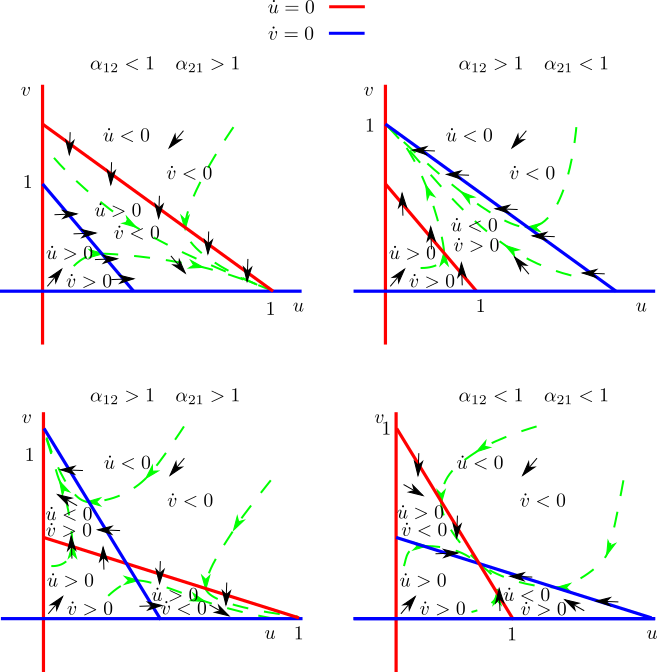
\includegraphics[width=\tp]{../../Pictures/Competitive_exclusion.png}
\caption{Phase planes in all possible configurations.\label{Phase_plane}}
\end{figure}
From the bottom left sketch of \fig{Phase_plane} we see that when $\alpha_{12},\alpha_{21}>1$ $(u_s,v_s)$ is unstable, specifically, it is a saddle point. Equally, the bottom right sketch of \fig{Phase_plane} shows that when $\alpha_{12},\alpha_{21}<1$ $(u_s,v_s)$ is stable.

\item In this model we see four possible outcomes. In three of these cases only one of the populations survives and exists at the expense of the other, \eg the red squirrel population survives, but the grey squirrel population dies out. Only in the case that $\alpha_{12},\alpha_{21}<1$ are both populations able to live together. In ecology this concept is called competitive exclusion. It suggests that two species competing for exactly the same resources cannot stably coexist. One of the two competitors will always have an ever so slight advantage over the other that leads to extinction of the second competitor in the long run (or evolution into distinct ecological niches).

\item \fig{SquirrelMap} shows that the squirrels are being pushed further and further north. Thus, it seems like the grey squirrels are winning out, thus, we would expect to be in the case that at least (1,0) is stable, \ie $\alpha_{21}>1$.

\item First we need $(u_s,v_s)$ to exist and be stable. This work has already been done above and, thus, we are in the case that $\alpha_{12},\alpha_{21}<1$. Then either by linearising the system using a perturbation of the form
\bb
\l \begin {array}{c} u\\ v
\end {array} \r
=
\frac{1}{1-\alpha_{12}\alpha_{21}}\l \begin {array}{c} 1-\alpha_{12}\\ 1-\alpha_{21}
\end {array} \r
+
\l \begin {array}{c} \epsilon_1\\ \epsilon_2
\end {array} \r
\exp(\lambda t)\cos(kx),
\ee
or by writing the Turing inequalities down we find that we need to satisfy
\bb
g_v+Df_u>2\sqrt{D(f_ug_v-f_vg_u)},
\ee
substituting in $f=u(1-u-\alpha_{12})$ and $g=\rho v(1-v-\alpha_{21}u)$ and the steady state $(u_s,v_s)$ we derive
\bb
\frac {1}{\alpha_{12}\alpha_{21}-1} \l  2\l 1 -\alpha_{12}\alpha_{21} \r \sqrt{{\frac{D\rho \l 1-\alpha_{12}\r \l 1-\alpha_{21} \r }{1-\alpha_{12}\alpha_{21}}}}+D(1-\alpha_{12})+\rho(1-\alpha_{21}) \r >0.
\ee
Since $\alpha_{12},\alpha_{21}<1$ the $\alpha_{12}\alpha_{21}-1<0$ and, so,
\bb
  \UB{2\l 1 -\alpha_{12}\alpha_{21} \r \sqrt{{\frac{D\rho \l 1-\alpha_{12}\r \l 1-\alpha_{21} \r }{1-\alpha_{12}\alpha_{21}}}}}{$>0$}+\UB{D(1-\alpha_{12})}{>0}+\UB{\rho(1-\alpha_{21})}{>0} <0.\label{ineq}
\ee
However, as shown in inequality \eqref{ineq}, all the terms on the left-hand side are positive, thus, the inequality cannot be satisfied, meaning that the interacting squirrel model cannot produce Turing patterns.

\item $D=1$ means that both squirrel populations spread out at the same rate. $\rho=1$ means that the interaction time scales are the same. Namely, each interactions takes the same time. $\alpha_{12}=1/2<3/2=\alpha_{21}$ means that the grey squirrels out compete the red squirrels 3 out of 4 times. The initial condition means that we are initially in a system that is full of red squirrels only. However, the boundary conditions means that grey squirrels are being released at $x=-\infty$ and red squirrels are being destroyed. Equally, at $x=\infty$ red squirrels are being released and grey squirrels are being destroyed. Of course an infinitely long domain is physically impossible. The domain size just has to be large compared to the movement length scale of the squirrels.

\item Considering the results above heterogeneous patterning will not occur and the parameter values put us in the case of (0,0), (0,1) and $(u_s,v_s)$ being unstable, whilst (1,0) is stable. Namely, since the grey squirrels out compete the red we expect that the grey squirrels will invade the entire territory and wipe the red squirrels out.

\item using $z=X-c\tau$ means that
\bb
\D{}{X}=\D{}{z}\D{z}{X}=\D{}{z}.
\ee
and
\bb
\D{}{\tau}=\D{}{\tau}\D{\tau}{\tau}+\D{}{z}\D{z}{\tau}=\D{}{\tau}-c\D{}{z}.
\ee
Upon substitution we generate
\begin{align}
\D{u}{\tau}-c\D{u}{z}=&\DD{u}{z}+u\l 1-u-\frac{1}{2}v\r,\label{uz}\\
\D{v}{\tau}-c\D{v}{z}=&\DD{v}{z}+v\l 1-v-\frac{3}{2}u\r.\label{vz}
\end{align}



\item First, we are dealing with a stationary profile in the travelling frame of reference so derivatives with respect to $\tau$ disappear. Now we add together \eqns{uz}{vz} to get
\bb
0=\DD{u+v}{z}+c\D{u+v}{z}+u+v-2uv-u^2-v^2.
\ee
Letting $s=u+v$ this simplifies to
\bb
0=\DD{s}{z}+c\D{s}{z}+s-s^2.
\ee
The boundary conditions and initial conditions are $s(-\infty,t)=s(\infty,t)=s(x,0)=1$.

\item $s\equiv 1$

\item Since $1=s=u+v$ we can substitute $v=1-u$ into \eqn{uz}. Rearranging and cancelling the $\tau$ derivative once again leads to \eqn{u_solo}.

\item To show a travelling wave is possible we need to consider the stability of $u=0$ and $u=1$. Since $u$ corresponds to grey squirrels we expect the wave to invade from the $u=1$ boundary towards the $u=0$ boundary. Thus, we need to show that $u=0$ is stable and $u=1$ is unstable. First we perturb around $u=0$ with $u=\epsilon\exp(\lambda z)$. Substituting this into \eqn{u_solo} gives
\bb
0=\lambda^2+c\lambda+1-\alpha_{12}.
\ee
So,
\bb
2\lambda_\pm=-c\pm\sqrt{c^2-4(1-\alpha_{12})}.
\ee
As mentioned we need $u=0$ to be stable, implying Re$(\lambda_\pm)<0$. Further, because $u$ is a physical population, $u>0$. Thus, $u=0$ cannot be a spiral point. Hence, the eigenvalues must be real and negative implying that $1>\alpha_{12}$, which is already satisfied, and $c^2-4(1-\alpha_{12})>0$, or $c> 2\sqrt{(1-\alpha_{12})}$.

We next check the stability of $u=1$ using $u=1+\epsilon\exp(\lambda t)$
\bb
0=\lambda^2+c\lambda-1+\alpha_{12}.
\ee
So,
\bb
2\lambda_\pm=-c\pm\sqrt{c^2+4(1-\alpha_{12})}.
\ee
Since $\alpha_{12}<1$ we have that $\lambda_-<0<\lambda_+$ and, thus, $u=1$ is unstable. Thus, a travelling wave with a stationary profile can exist.



\item The suggested model dynamics are that due to grey squirrels being ``fitter'' (in a Darwinian sense) than the red squirrels we should see a travelling wave of grey squirrel population pushing the red squirrel out. This is what is seen in \fig{SquirrelMap} between 1945 and 2000. However, after 2000 the wave seems to halt. This is due to conservation programmes that enable the red squirrel population to survive in certain carefully protected regions. Such external conservation factors are not included in the above model.
\end{enumerate}
\end{Answ}

\section{Amoebae movement}\label{Amoebae movement}
The amoebae of the slime mould \textit{Dictyostelium discoideum} secretes a chemical attractant, cyclic-AMP. The attractant diffuses away from the amoebae source and attracts other amoebae to it, causing spatial aggregations to form, see \fig{Dictyo} and the linked YouTube video.
\begin{figure}[h!!!tb]
\centering
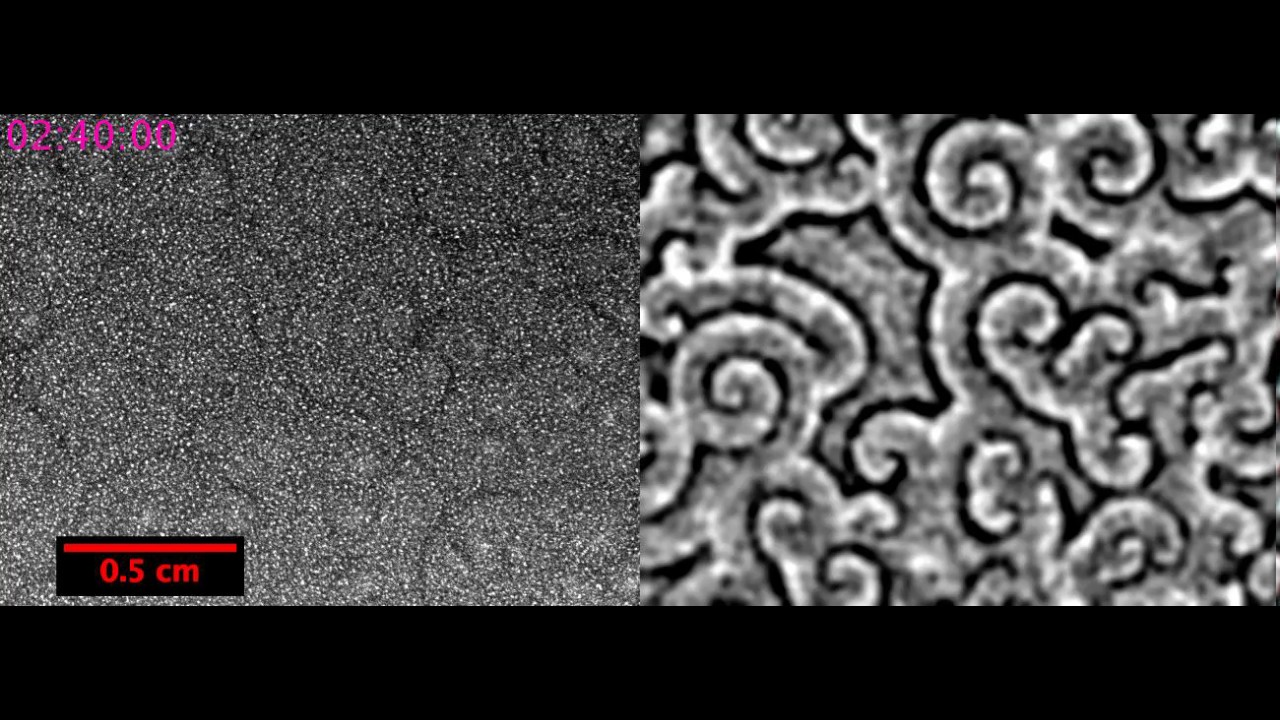
\includegraphics[width=\textwidth,trim={0cm 4cm 0cm 4cm},clip]{../../Pictures/Dictyo_pattern.jpg}
\caption{\label{Dictyo} Single frame of the a spatio-temporal wave pattern made by Dictyostelium discoideum. The full video can be found on \href{https://www.youtube.com/watch?v=oYRF7BaaaJY}{YouTube}. Have a watch to see how the pattern is generated from randomness.}
\end{figure}

In the following assume that we are on a infinite, one-dimensional domain so that we can be loose with boundary conditions.

The attractant (concentration denoted $a$) is secreted by the amoebae (concentration denoted $n$) at a rate proportional to the amoebae concentration. The attractant is able to diffuse and the attractant decays at a rate proportional to the attractant's concentration.
\begin{enumerate}
\item Justify the following equation for the attractant population,
\bb
\D{a}{t}=D_a\DD{a}{x}+k_1n-k_2a.
\ee
\setcounter{Counter1}{\value{enumi}}
\end{enumerate}

The amoebae do not reproduce or degrade, however, alongside their diffusive motion (\fig{Diffusive_motion}) they also undergo attractant controlled motion (chemotaxis, as shown in \fig{Attractant_controlled_motion}) .
\begin{figure}[h!!!tb]
\centering
\subfigure[\label{Diffusive_motion}Schematic of diffusive motion]{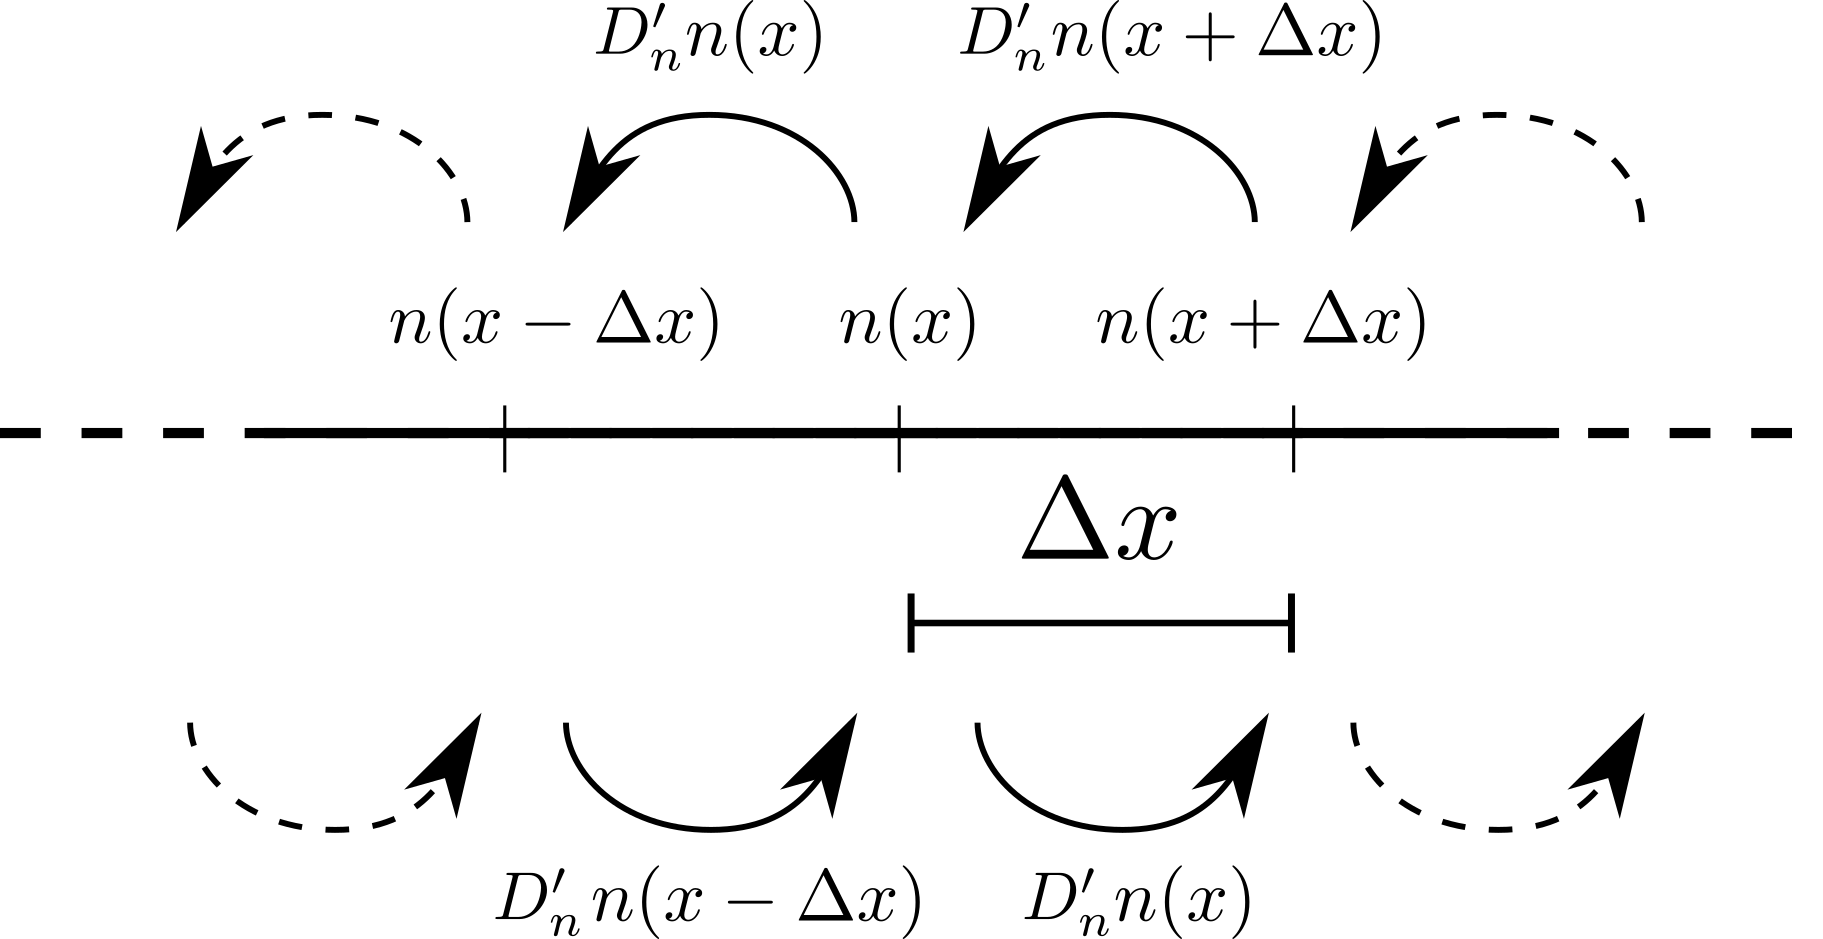
\includegraphics[width=\ttp]{../../Pictures/Diffusive_motion.png}}\\
\subfigure[\label{Attractant_controlled_motion} Schematic of chemotaxis]{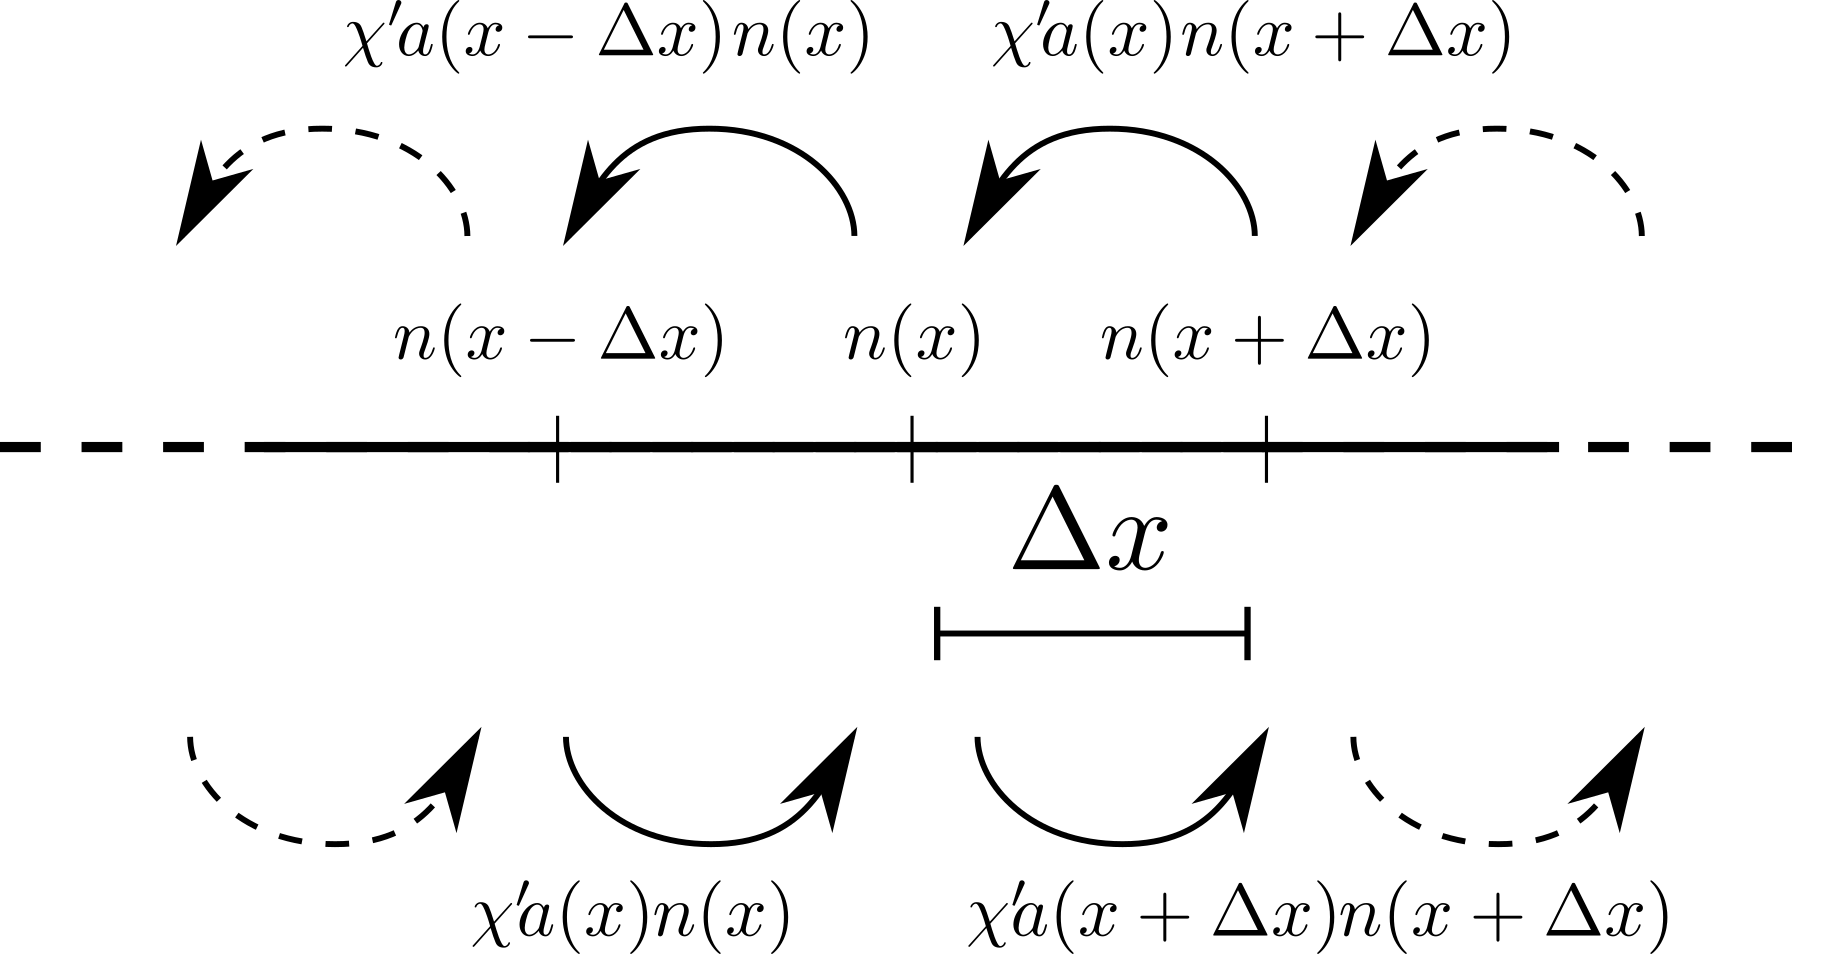
\includegraphics[width=\ttp]{../../Pictures/Attractant_controlled_motion.png}}
\caption{\label{Motion_types} Different motion types of the amoebae.}
\end{figure}

\begin{enumerate}
\setcounter{enumi}{\value{Counter1}}
\item Using the process of considering an infinite discretised domain, derive the equation of the amoebae movement. Show that, upon taking a continuum spatial limit the equations can be simplified to
\bb
\D{n}{t}=D_n\DD{n}{x}-\chi\D{}{x}\l n\D{a}{x}\r.
\ee
where $D_n$ and $\chi$ should be defined in terms of $D'_n$, $\chi'$ and $\Delta x$.
\setcounter{Counter1}{\value{enumi}}
\end{enumerate}

We now consider the system
\begin{align}
&\D{n}{t}=D_n\DD{n}{x}-\chi\D{}{x}\l n\D{a}{x}\r,\label{n}\\
&\D{a}{t}=D_a\DD{a}{x}+n-a.\label{a}
\end{align}
where we have set $k_1=1=k_2$. The system is on an infinite one-dimensional domain. The boundary conditions are zero-flux and the initial conditions are uniformly distributed random perturbations about a mean of $n=a=1$ and range 1/10.
\begin{enumerate}
\setcounter{enumi}{\value{Counter1}}
\item What is the spatially homogeneous steady states $(n_s,a_s)$ of system \eqref{n}-\eqref{a}?

\item Perturb around this homogeneous steady state using a spatial perturbation and derive conditions under which the homogeneous steady state will evolve to a patterned state.

\item Experimentally, $\chi$ is seen to increase during the life cycle of the slime mould. What does this mean? What would you expect to see over the course of the experiment?
\end{enumerate}

%\begin{figure}[h!!!tb]
%\centering
%\includegraphics[width=\textwidth]{../../Pictures/Movement_schematic.png}
%\caption{\label{SquirrelMap} Schematic of amoebae movement patterns.}
%\end{figure}


\begin{Answ}
\subsection{Answers}
\begin{enumerate}
\item 
\bb
\UB{\D{a}{t}}{Evolution of the morphogen}=\UB{D_a\DD{a}{x}}{Diffusion of the morphogen}+\UB{k_1n}{Creation of the morphogen}-\UB{k_2a}{Degradation of the morphogen}.
\ee


\item From \fig{Motion_types} we can right down the evolution of $n_i=n(x)$ in terms of $n_{i\pm 1}=n(x\pm\Delta x)$ and $a_{i\pm 1}=a(x\pm\Delta x)$,
\bb
\dot{n}_i=D'_n\l n_{i-1}-2n_i+n_{i+1}\r+\chi' \l a_in_{i+1}-a_{i-1}n_i+a_in_i-a_{i+1}n_{i+1} \r.
\ee
Using
\bb
u_{i\pm1}=u_i\pm \D{u_i}{x}+\frac{1}{2}\DD{u_i}{x}+O(\Delta x^3)
\ee
to expand all the terms we find that
\bb
\dot{n}_i=D'_n\Delta x^2 \DD{n_i}{x}-\chi'\Delta x^2 \l n_i\DD{a_i}{x}+\D{n_i}{x}\D{a_i}{x} \r.
\ee
Letting $D_n=D'_n\Delta x^2$ and $\chi=\chi'\Delta_x^2$ be finite we take $\Delta x\rightarrow 0$ and simplify to
\bb
\D{n}{t}=D_n\DD{n}{x}-\chi\D{}{x}\l n\D{a}{x}\r.
\ee

\item Searching for the homogeneous steady state means we ignore all derivatives. However, that means \eqn{n} does not provide any information. However, the zero-flux boundary conditions means that the $n$ population is neither created, degraded, nor is it able to leave the domain. Thus, the homogeneous steady state is found by averaging out the total initial density across the entire domain,
\bb
n_s=\lim_{L\rightarrow \infty}\frac{1}{2L}\int^L_{-L} n(x,0) \rd x.
\ee
Call this $n_0$.
From \eqn{a} we find that the steady state satisfies $a_s=n_s=n_0$.

\item We substitute the perturbation
\bb
\l\begin{array}{c}
n\\
a
\end{array}\r
=
\l\begin{array}{c}
n_0\\
n_0
\end{array}\r
+
\l\begin{array}{c}
\epsilon_1\\
\epsilon_2
\end{array}\r\exp(\lambda t)\cos(kx).
\ee
into \eqns{n}{a} and derive
\begin{align}
\lambda\cos(kx)\exp(\lambda t)\l\begin{array}{c}
\epsilon_1\\
\epsilon_2
\end{array}\r
=
-k^2\cos(kx)\exp(\lambda t)\l\begin{array}{cc}
D_c & 0\\
0 & D_a
\end{array}\r\l\begin{array}{c}
\epsilon_1\\
\epsilon_2
\end{array}\r
+
\cos(kx)\exp(\lambda t)\l\begin{array}{c}
n_0\chi k^2\epsilon_2\\
\epsilon_1-\epsilon_2
\end{array}\r.
\end{align}
Upon simplification
\bb
\l\begin{array}{cc}
-k^2D_c-\lambda & n_0\chi k^2\\
1 & -k^2D_a-\lambda-1
\end{array}\r\l\begin{array}{c}
\epsilon_1\\
\epsilon_2
\end{array}\r=\bm{0}.
\ee
We now invoke the result that the determinant of the matrix must be zero in order to have a non-trivial solution for $(\epsilon_1,\epsilon_2)$. Thus,
\bb
0=(-k^2D_c-\lambda)(-k^2D_a-\lambda-1)-n_0\chi k^2=\lambda^2+\lambda(k^2D_a+k^2D_c+1)+k^4D_cD_a+k^2(D_c-n_0\chi).
\ee
For an instability to happen at least one root, $\lambda$, must be positive,
\bb
2\lambda_\pm=-(k^2D_a+k^2D_c+1)\pm\sqrt{(k^2D_a+k^2D_c+1)^2-4\l k^4D_cD_a+k^2(D_c-n_0\chi)\r}.
\ee
Thus, we require
\bb
0>k^4D_cD_a+k^2(D_c-n_0\chi)=k^2D_cD_a\l k^2+\frac{(D_c-n_0\chi)}{D_cD_a}\r.\label{Quad_k}
\ee
Since inequality \eqref{Quad_k} is a positive quartic then we need
\bb
\frac{(D_c-n_0\chi)}{D_cD_a}<0, \implies D_c<n_0\chi
\ee

\item $\chi$ is the chemotactic parameter, increasing it means that the cells become more attracted to the diffusing morphogen. Thus, even if initially the cells do not pattern eventually $\chi$ will increase to a point that satisfies the condition $D_c<n_0\chi$. Thus, the population will eventually pattern.
\end{enumerate}

\end{Answ}



\end{document}